% arara: pdflatex
% !arara: animate: {delay: 80}
% !arara: indent: {overwrite: yes, localSettings: yes}
\documentclass[aspectratio=43,mathserif]{beamer}
%\documentclass[handout,mathserif]{beamer}
\usepackage{caption}
\usepackage{amsmath}
\usepackage{booktabs}
\usepackage{etoolbox}
\usepackage{multirow}
\usepackage{pgfplots}
\usepackage[]{media9}
\usepackage{mathtools}
\usetikzlibrary{positioning}
\usetikzlibrary{fit}
\usetikzlibrary{backgrounds}
\usetikzlibrary{calc}
\usetikzlibrary{shapes}
\usetikzlibrary{mindmap}
\usetikzlibrary{decorations.text}
\pgfplotsset{compat=1.7}
\let\bbordermatrix\bordermatrix
\patchcmd{\bbordermatrix}{8.75}{4.75}{}{}
\patchcmd{\bbordermatrix}{\left(}{\left[}{}{}
\patchcmd{\bbordermatrix}{\right)}{\right]}{}{}

\usepackage[english]{babel}

\usepackage[style=mla,backend=bibtex]{biblatex}

\usetheme[titlepagelogo=figures/fer,
  secondlogo = true,
  thirdlogo = true,
  color=larics,
  language=custom,
  bullet=square,
  ]{TorinoTh}
  
\titlepagesecondlogo{figures/unizg}
\titlepagethirdlogo{figures/larics_light}
\author{mag. ing. Lovro Markovic}
\setcandidatelabel{Candidate}
\setrellabel{Supervisor}
\setsubject{PhD Qualifying Exam}
\rel{prof. dr. sc. Stjepan Bogdan}
\title[PhD Qualifying Exam]{State-of-the-Art Survey of Manifold Based Control Methods for	Unmanned Aerial Vehicles}

\ateneo{Faculty of Electrical Engineering and Computing, University of Zagreb}
\date{Zagreb, 9.3.2020.}
\usepackage{subfigure}
\usepackage{multirow}
\newcommand{\backupbegin}{
   \newcounter{framenumberappendix}
   \setcounter{framenumberappendix}{\value{framenumber}}
}
\newcommand{\backupend}{
   \addtocounter{framenumberappendix}{-\value{framenumber}}
   \addtocounter{framenumber}{\value{framenumberappendix}} 
}

% tikzmark command, for shading over items
\newcommand{\tikzmark}[1]{\tikz[overlay,remember picture] \node (#1) {};}

% standard enumeration
%\setbeamertemplate{enumerate items}{(\arabic{enumi})}

% default itemize
\setbeamertemplate{itemize items}[circle]

% transparency
\setbeamercovered{transparent=15}

% for resuming lists across frames
\newcounter{savedenum}
\newcommand*{\saveenum}{\setcounter{savedenum}{\theenumi}}
\newcommand*{\resume}{\setcounter{enumi}{\thesavedenum}}

% title
\tikzset{
   invisible/.style={opacity=0},
   visible on/.style={alt=#1{}{invisible}},
   alt/.code args={<#1>#2#3}{%
      \alt<#1>{\pgfkeysalso{#2}}{\pgfkeysalso{#3}} % \pgfkeysalso doesn't change the path
   },
}

%\includeonlyframes{daytoday}

% add references
\addbibresource{./bibliography/Mendeley.bib}

\begin{document}
\begin{frame}[plain, noframenumbering]
\titlepage
\end{frame}

\begin{frame}
	\frametitle{Table of Contents}
	\tableofcontents
\end{frame}

\AtBeginSection[]
{
	\begin{frame}<beamer>
		\frametitle{Table of Contents}
		\tableofcontents[currentsection]
	\end{frame}
}


\section{Introduction}

\begin{frame}
	\frametitle{Research Area}
	
	\begin{itemize}
		\item Unmanned Aerial Vehicles (UAVs)
		\item Attitude $(\phi, \theta, \psi)$ and Position $(x, y, z)$ control
		\item Mathematical model embedded with a manifold structure
		\item Two frameworks considered:
		
		\begin{itemize}
			\item Geometric Mechanics and Control
			\item Passive Decomposition
		\end{itemize}
	\end{itemize}
\end{frame}

\begin{frame}
	\frametitle{Which Manifolds?}
	
	\begin{itemize}
		\item UAV configuration space:
	\end{itemize}
	\begin{equation*}
		\zeta = [x, y, z, \phi, \theta, \psi] \in \mathbb{R}^6 
		\xleftrightarrow[f_{\zeta_0}^{-1}(\zeta)]{f_{\zeta_0}(\zeta)}
		\begin{bmatrix}
		\text{R} & \textbf{p} \\
		\textbf{0} & 1
		\end{bmatrix}_{4\times 4} \in \text{SE(3)} \, , \; \text{R} \in \text{SO(3)}
	\end{equation*}
	
	\begin{itemize}
		\item Lie Group
		\begin{itemize}
			\item set of smooth differentiable manifolds
			\item group multiplication and inversion properties
			\item e.g. SO(3), SE(3), $\text{S}^2$
		\end{itemize}
	\end{itemize}
\end{frame}

\begin{frame}
	\frametitle{Why manifolds?}
	
	\begin{itemize}
		\item Compact model dynamics represented as a Lagrangian / Hamiltonian system
		\item Coordinate-free approach
		\item No singularities
		\item No ambiguities
	\end{itemize}
\end{frame}
\section{Geometric Control and Mechanics}

\begin{frame}
	\frametitle{Geometric Mechanics}
	
	\begin{itemize}
		\item Introduced by:
		\begin{itemize}
			\item F. Bullo and A. Lewis, 2005. \footcite{bulloBook}
			\item T. Lee, 2008. \footcite{Lee2008ComputationalGM}
			%\footcite{Taeyoung Lee, Computational geometric mechanics and control of rigid bodies}
			\item T. Lee et al. 2018. \footcite{LeeModel} 
		\end{itemize}
	
	\end{itemize}
	\begin{itemize}
		\item Rotating rigid body dynamics equation:
	\end{itemize}	
	\begin{equation}
		m \ddot{\textbf{x}} + m g\textbf{e}_3 = f\text{R}\textbf{e}_3 \label{model1}
	\end{equation}
	\begin{equation}
		\text{J}\dot{\mb{\Omega}} + \mb{\Omega} \times \text{J}\mb{\Omega} = \textbf{M} \label{model2}
	\end{equation}
	\begin{equation}                       
		\dot{\text{R}} = \text{R}\widehat{\mb{\Omega}} \label{model3}
	\end{equation}
	
\end{frame}

\begin{frame}
	\frametitle{Geometric Control (1)}

	\begin{itemize}
		\item PD control with nonlinear terms
		\item First developed by T. Lee et al. 2010. \footcite{LeeClanak4}
		\item Robust variant by T. Lee et al. 2011. \footcite{LeeClanak3}
		\item L1 Aadaptive controller by Kotaru et al. 2019. \footcite{Kotaru2019GeometricLA}
		\item Parameter tuning optimization by S. Lee et al. 2019. \footcite{Lee2019}
	\end{itemize}
\end{frame}

\begin{frame}
	\frametitle{Geometric Control (2) \footcite{Markovic2019}}
	
	\begin{columns}
		\begin{column}{0.5\textwidth}\centering
			\begin{figure}[H]
				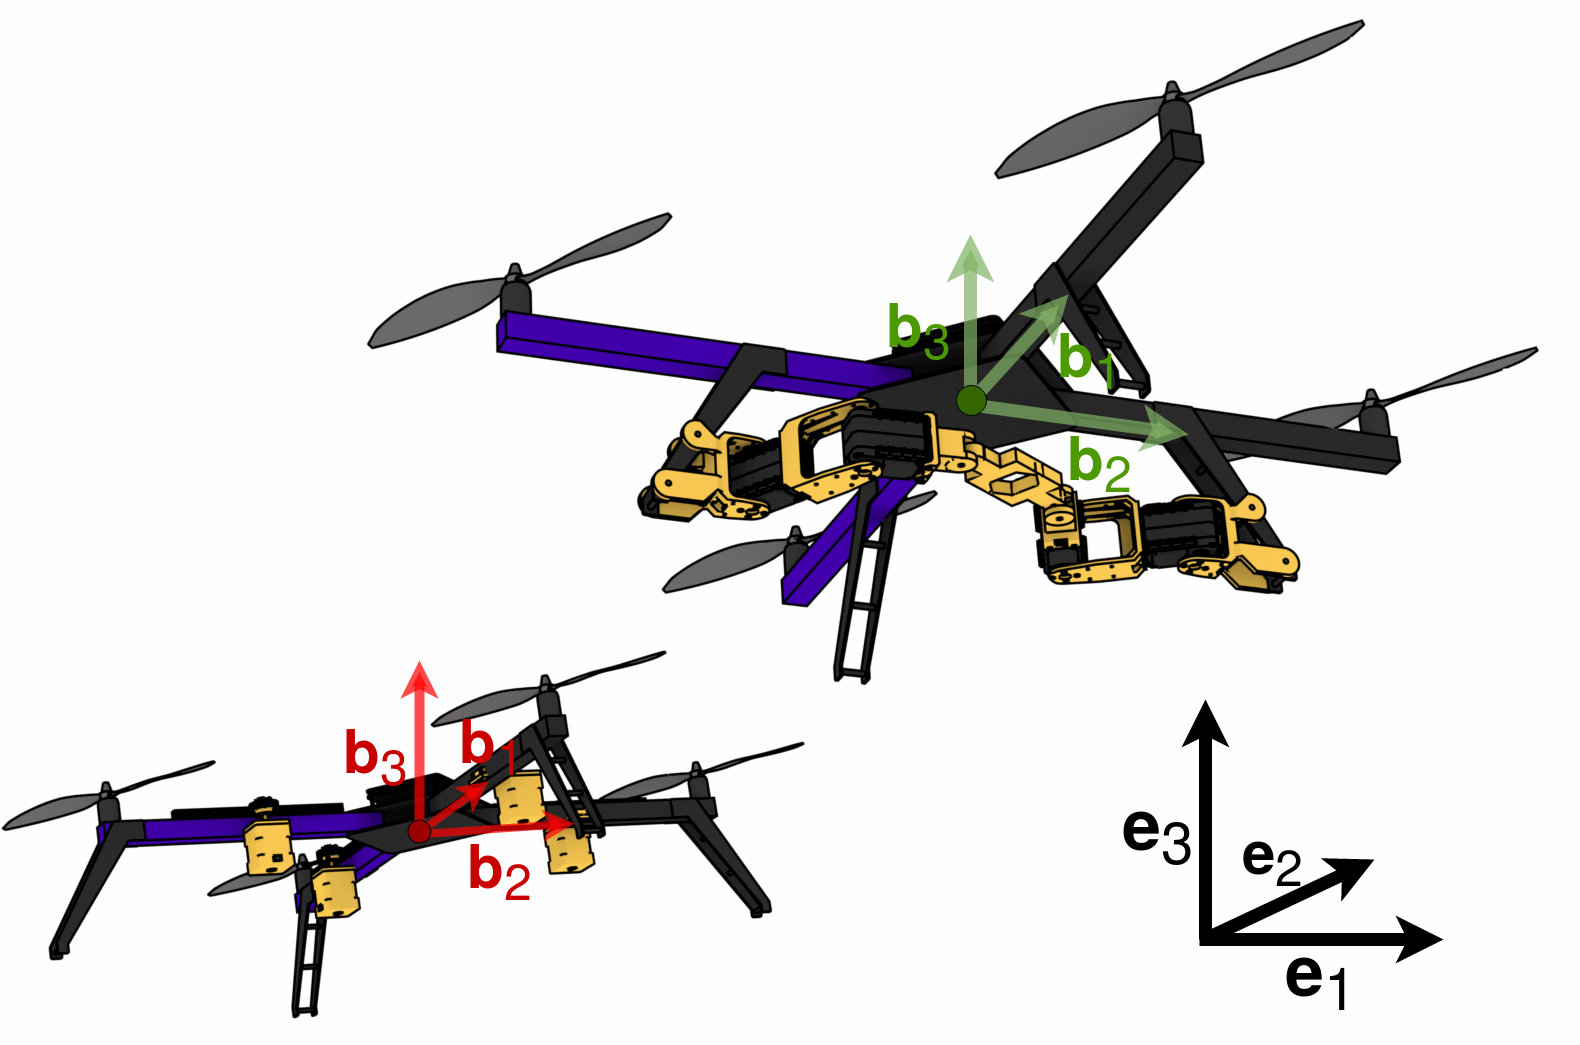
\includegraphics[width=0.8\columnwidth]{figures/uav.png}	
				\centering
				\caption{Two UAVs endowed with variable center of gravity by moving masses and manipulator carried payload (top). Position tracking results (right)${}^{8}$. }
				\label{fig:uav_model}
			\end{figure}
		\end{column}
		
		\begin{column}{0.5\textwidth}\centering
			\begin{figure}
				\centering
				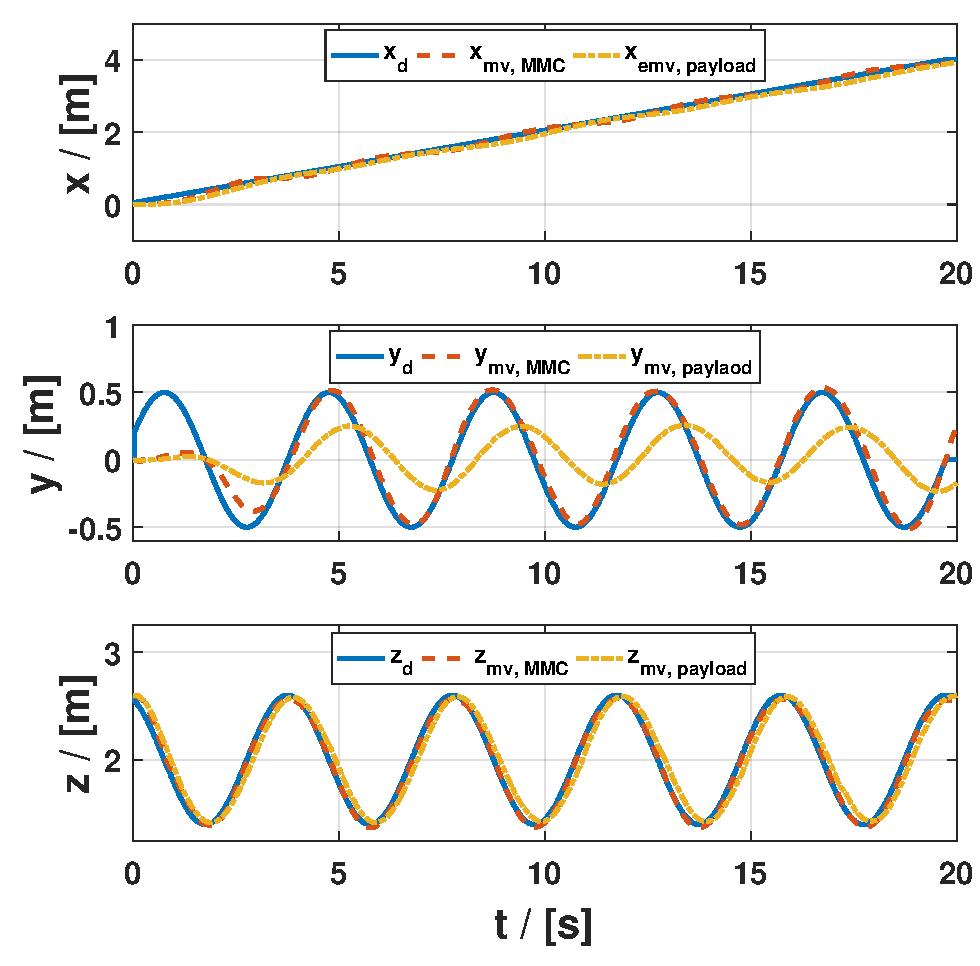
\includegraphics[width=0.95\columnwidth]{figures/both_pos_crop.pdf}
				\label{fig:traj_pos}
			\end{figure}
		\end{column}
	\end{columns}
\end{frame}

\begin{frame}
	\frametitle{Gemetric Control - Transportation Tasks (1)}
	
	\begin{itemize}
		\item Introduced by T. Lee and V. Kumar 2013. \footcite{cable-load1}
		\item Variations with multiple quadrotors presented by A. Goodarzi and T. Lee 2015. \footcite{cable-load-multiple}
		\item Adaptive control with unknown mass variations by A. Goodarzi and T. Lee 2015 \footcite{flexible-cable-dynamics} and A. Goodarzi et al. 2013. \footcite{stabilization-flexible-cable}
	\end{itemize}
\end{frame}

\begin{frame}
	\frametitle{Geometric Control - Transportation Tasks (2) \footcite{Lee2014GeometricCO}}
	
	\begin{columns}
		\begin{column}{0.5\textwidth}\centering
			\begin{itemize}
				\item Multiple quadrotor UAVs carrying a rigid body payload via cables
				\item Cable configuration is defined in $\text{S}^2$ - spherical Lie group
				\item Complete system configuration is defined by $\text{SE(3)} \times \text{S}^2$
				\item Payload position and attitude tracking problem
			\end{itemize}
		\end{column}
		
		\begin{column}{0.5\textwidth}\centering
			\begin{figure}[H]
				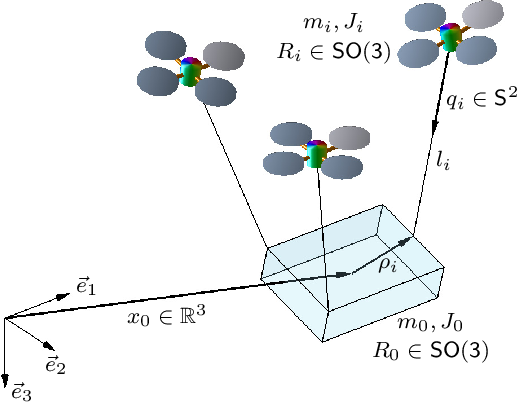
\includegraphics[width=0.9\columnwidth]{figures/payload_carrying.png}
				\caption{Payload transportation with multiple UAVs.${}^{13}$}
				\centering
			\end{figure}
		\end{column}
	\end{columns}
		
\end{frame}
\section{Passive Decomposition}

\begin{frame}
	\frametitle{Passive Decomposition}
	
	\begin{itemize}
		\item First introduced by D. Lee 2008. \footcite{LeePassive}
		\item Proposed system dynamics split:
		\begin{itemize}
			\item Shape	- internal configuration of each robot
			\item Locked - current overall behavior of multiple robot systems 
			\item Coupled - interaction between locked and shape dynamics
		\end{itemize}
		\item Passive decomposition
		\begin{itemize}
			\item Applying a control law to cancel the dynamics coupling terms without energy generation
			\item Enforces energetic passivity
		\end{itemize}
	\end{itemize}
\end{frame}

\begin{frame}
	\frametitle{Passive Decomposition - QM systems \footcite{passive-decomp-quadrotor-with-robotic-manip}$\,$  \footcite{decoupled-aerial-manipulation}}
	
	\begin{columns}
		\begin{column}{0.5\textwidth}\centering
			\begin{figure}[H]
				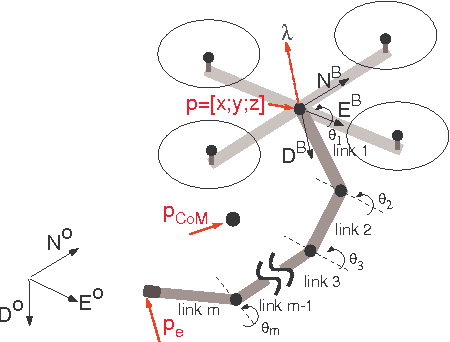
\includegraphics[width=0.9\columnwidth]{figures/aerial_manip.png}	
				\centering
				\caption{QM system${}^{15}$}
				\label{fig:aerial_manip}
			\end{figure}
		\end{column}
		
		\begin{column}{0.5\textwidth}\centering
			\begin{itemize}
			\item Decoupled quadrotor-manipulator(QM) system:
			\begin{itemize}
				\item center-of-mass dynamics in E(3)
				\item Robotic manipulator Lagrange dynamics
			\end{itemize}
			\item End-effector control law:
			\begin{itemize}
				\item Backstepping-like $\text{controller}^{16}$
				\item PID $\text{cascade}^{17}$
			\end{itemize}
			\end{itemize}
		\end{column}
	\end{columns}
 \end{frame}

\begin{frame}
	\frametitle{Passivity Based Control - Payload Transportation}
	\begin{itemize}
		\item C. Meissen et al. 2017. \footcite{passivity-based-formation-load} - General formation and internal control laws
		\item M E. Guerrero et al. 2015. \footcite{passivity-based-payload-minimum-swing} - An Interconnection and Damping Assignment - Passivity Based Control (IDA-PBC) for payload swing suppression
		\item P. Prajapati et al. 2019. \footcite{payload-and-human} - Master-slave transportation strategy with human-in-the-loop
	\end{itemize}
\end{frame}

\begin{frame}
	\frametitle{Passivity Based Control - Aerial Compliance (1)}
	
	\begin{itemize}
		\item E. Spyrakos et al. 2019. \footcite{passive-variable-impedance-compliant} - Manipulator passivity preservation control (PPC)
		\item Q. Delamare 2019. \footcite{quadrotor-itneraction-environment} - Exploiting physical contact to achieve flight maneuvers
		\item M. Schuster et al. 2019. \footcite{max-wrench-min-energy} - Energy efficient approach to maximum in-flight wrench generation
	\end{itemize}
\end{frame}

\begin{frame}
	\frametitle{Passivity Based Control - Aerial Compliance (2)}
	\begin{itemize}
		\item R. Rashad et al. 2019. \footcite{passivity-based-physical-interaction} - Passivity based control of a fully actuated UAV for aerial physical interaction near hovering
	\end{itemize}
	\begin{figure}[H]
		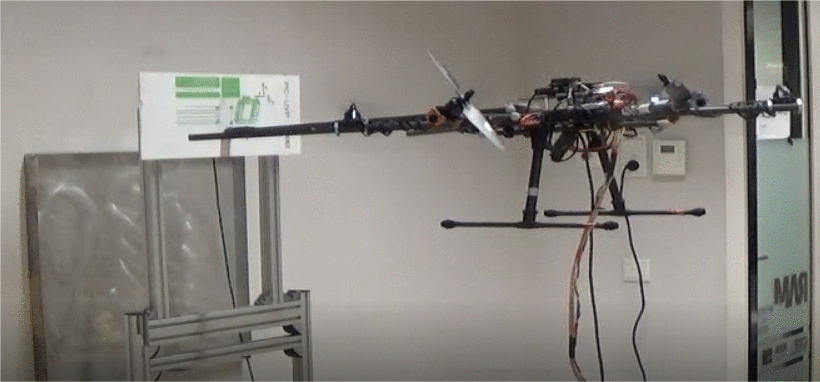
\includegraphics[width=0.6\columnwidth]{figures/passivity-based-interaction.png}	
		\centering
		\caption{A fully-actuated hexarotor UAV applying force to a vertical surface.}
		\label{fig:aerial_compliance}
	\end{figure}
 \end{frame}

\begin{frame}
	\frametitle{Passivity Based Control - Notable Mentions (1)}
	\begin{itemize}
		\item Y. Iarashi et al. 2009. \footcite{passivity-attitude-sync} 
		\begin{itemize}
			\item Passivity based motion coordination of rigid bodies by exchanging information over connected graphs
		\end{itemize} 
		\item H. Yang and D. Lee 2015. \footcite{cooperative-control-quadrotor}
		\begin{itemize}
			\item A hierarchical cooperative control framework
			\item Endowment of a common grasped object with desired behavior (e.g., trajectory tracking, compliant interaction, etc.)
		\end{itemize}
	\end{itemize}
\end{frame}

\begin{frame}
	\frametitle{Passivity Based Control - Notable Mentions (2)}
	\begin{itemize}
		\item P. Robuffo Giordano et al. 2011.\footcite{group-teleoperation} 
		\begin{itemize}
			\item Experimental validation of a decentralized passivity-based control strategy for teleoperating a group UAVs
			\item Master UAV (human-in-the-loop) controls the group motion and receives feedback about the remote slave motion status
		\end{itemize}
		\item D. Lee et al. 2013. \footcite{haptic-teleoperation-uav}
		\begin{itemize}
			\item Semi-autonomous haptic teleoperation control architecture for multiple UAVs
		\end{itemize}
	\end{itemize}
\end{frame}
\section{Conclusion}

\begin{frame}
	\frametitle{Future Work (1)}
	\begin{itemize}
		\item ENCORE project \footnote{"Encore project", http://encorebim.eu/ Accessed: 2019-09-10}
		\item Formation flight for building inspection
		\item Simultaneous exploration and physical interaction with architectural structures
		\item Applying passivity-based control in a real-world environment
		\item Goal: compliant multi-agent control method immune to communication unreliability while achieving energetic passivity
	\end{itemize}
\end{frame}

\begin{frame}
	\frametitle{Future Work (2)}
	\begin{itemize}
		\item Autonomous wind-turbine blade inspection using presented control frameworks
	\end{itemize}
	\begin{columns}
		\begin{column}{0.5\textwidth}\centering
			\begin{figure}[H]
				\centering
				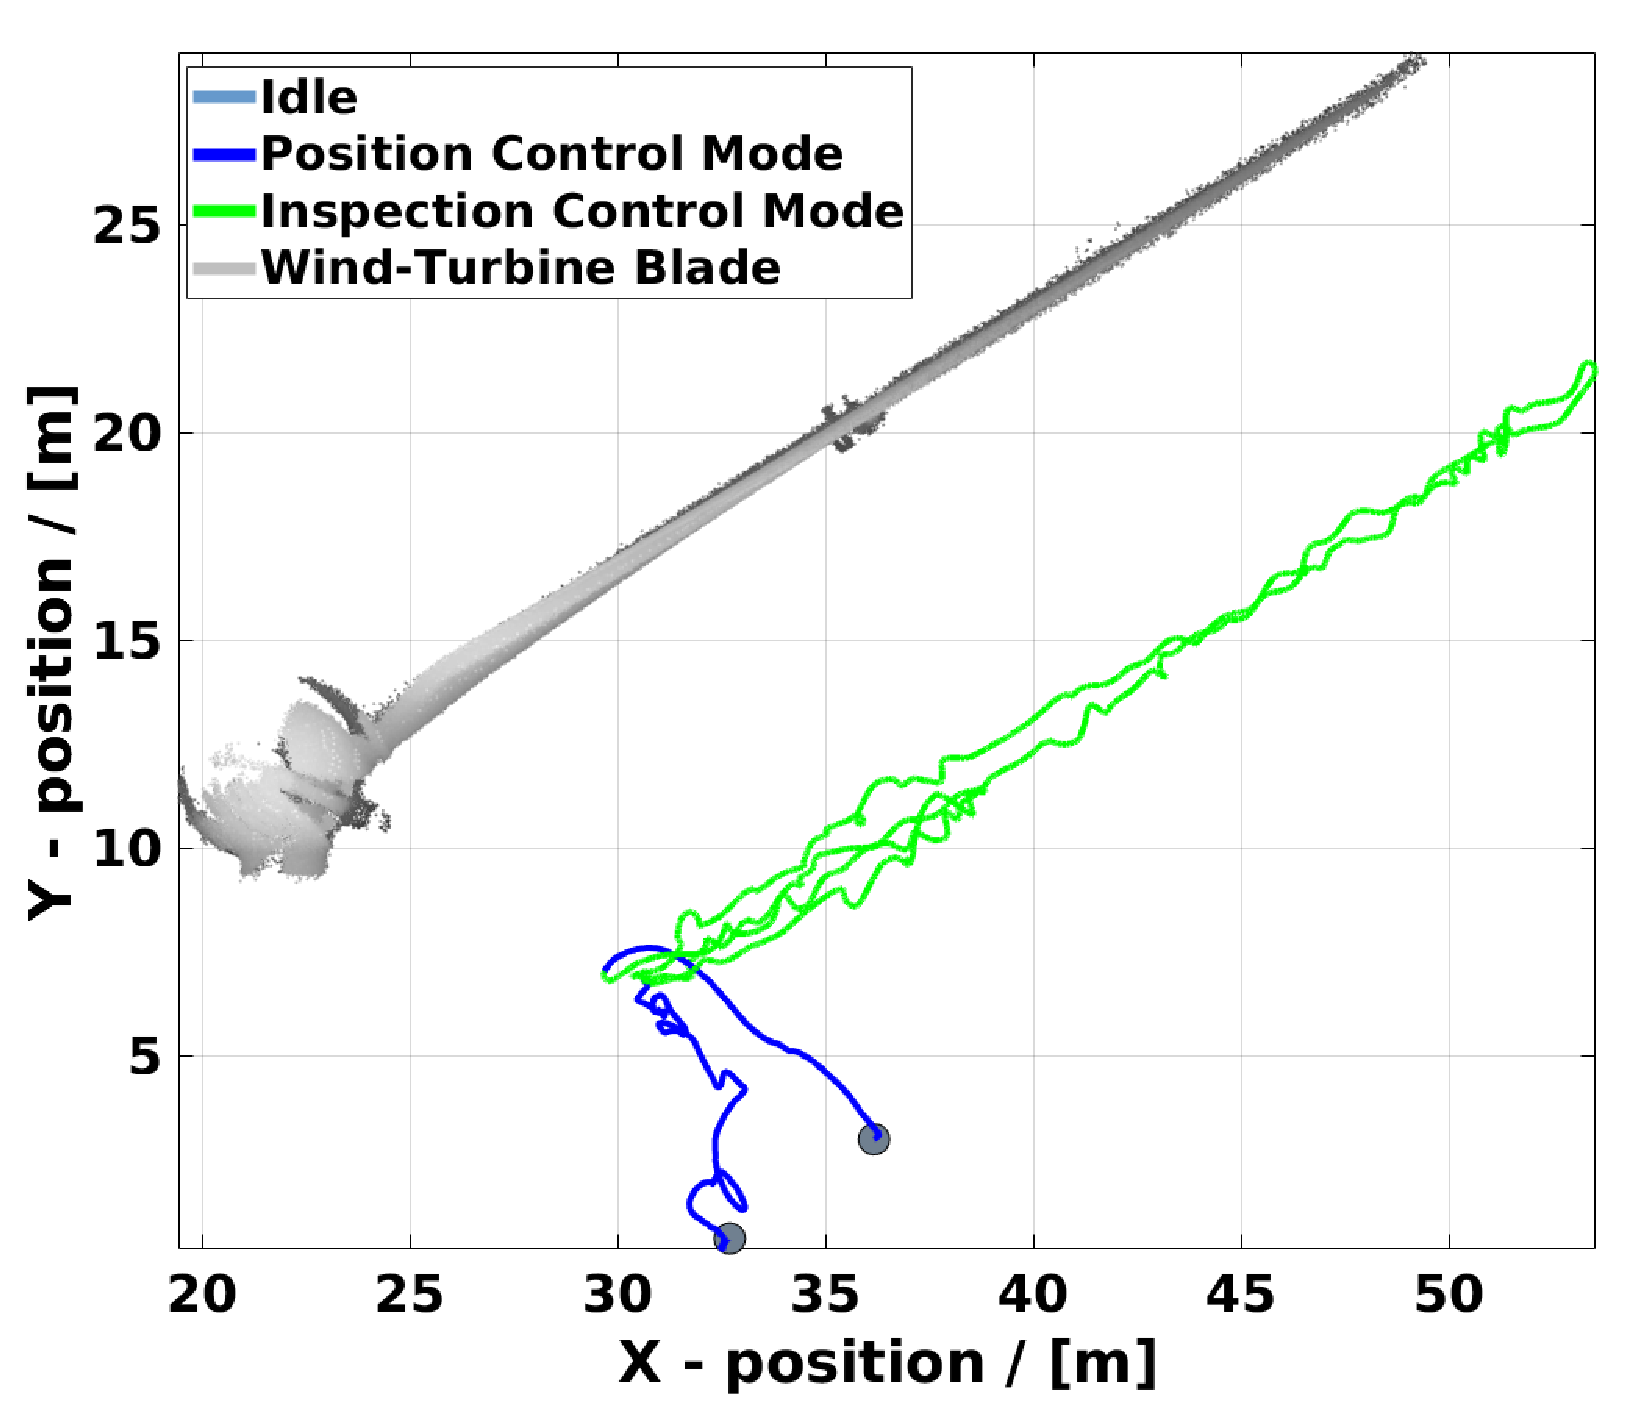
\includegraphics[width=0.8\columnwidth]{figures/uav_position_experiment_resized.pdf}
				\caption{Inspection trajectory and a wind-turbine model.}
				%\caption{Local position trajectory during the experimental wind-turbine blade inspection scenario \hlrevtwo{obtained from GPS measurements}. Blue and green colored trajectories show pilot-controlled position mode % and autonomous inspection control mode respectively. Slate gray colored markers represent takeoff and landing positions. \hlrevtwo{Wind-turbine blade model obtained post-inspection is shown as a reference.} }
			\end{figure}
		\end{column}
		\begin{column}{0.5\textwidth}\centering
			\href{video_presentation.mp4}{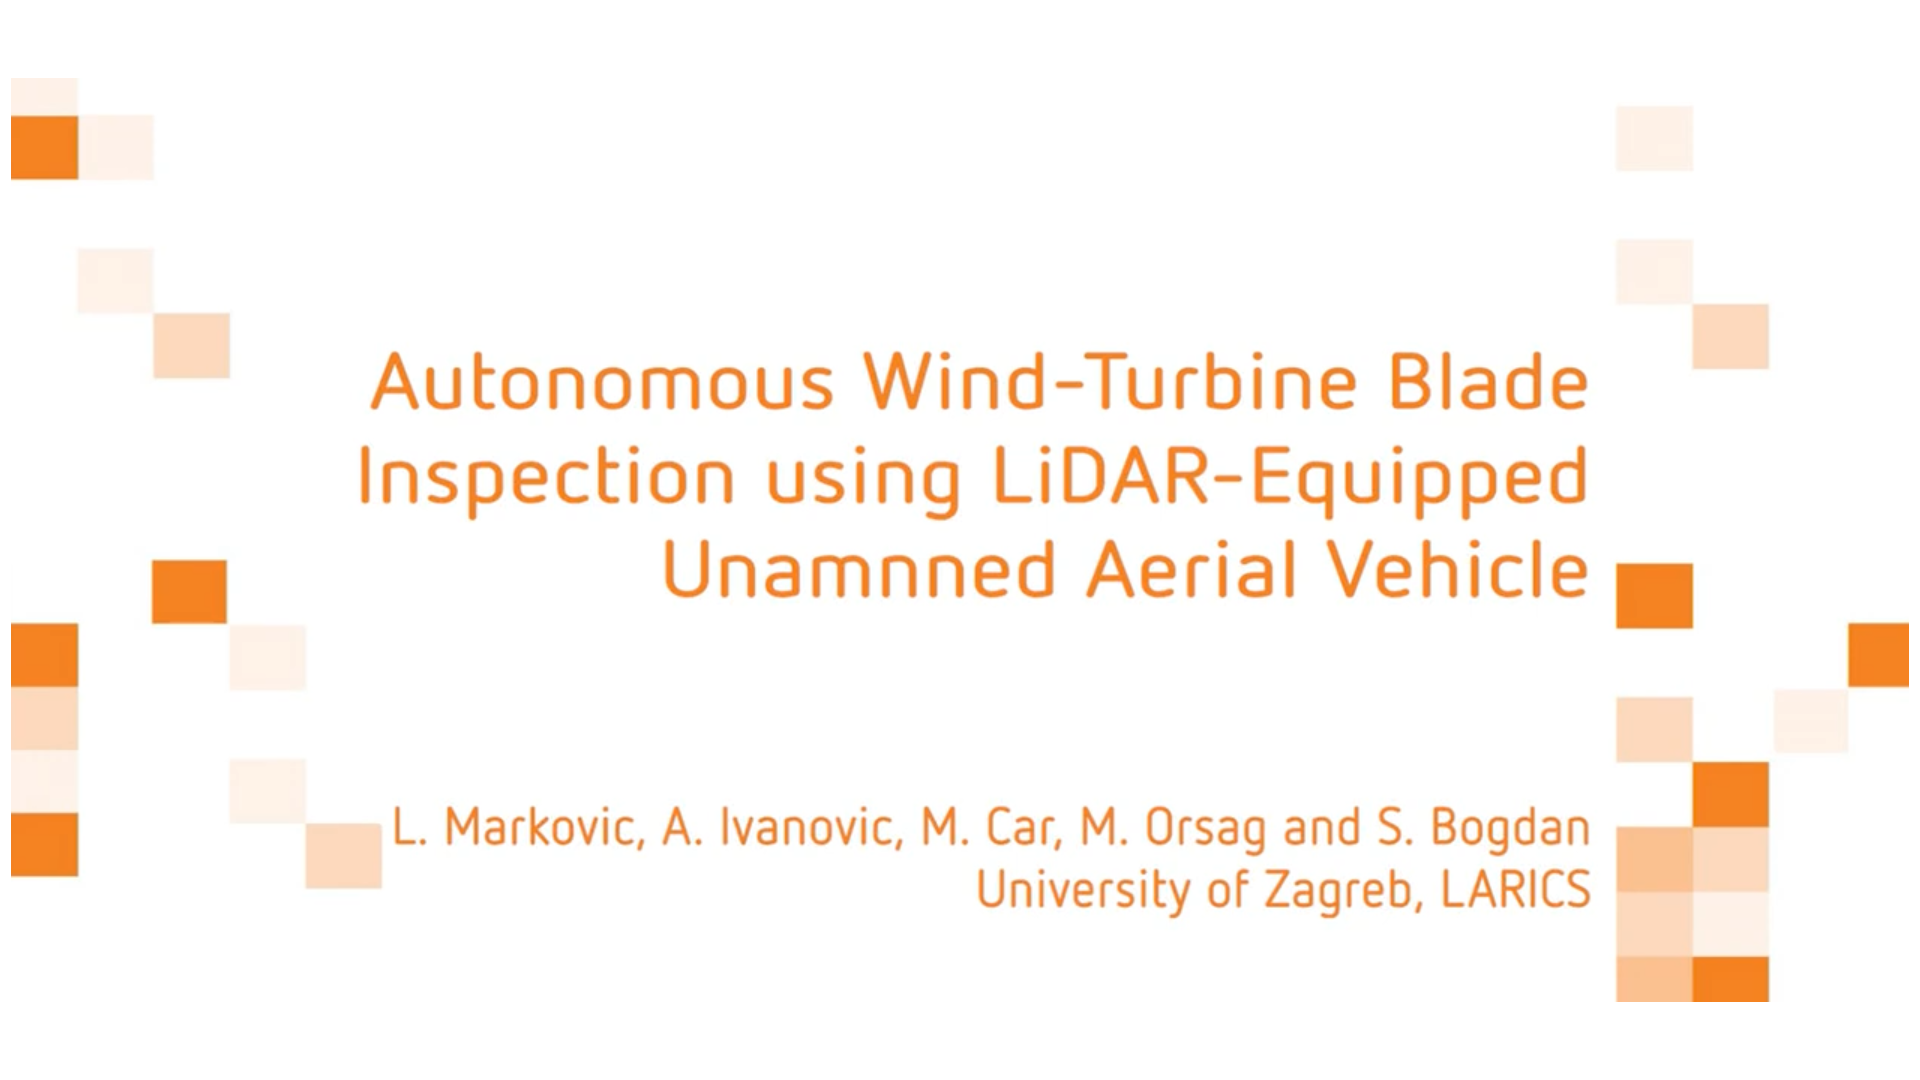
\includegraphics[width=\columnwidth]{figures/title_screen.png}}
		\end{column}
	\end{columns}
\end{frame}


\begin{frame}
	\frametitle{Conclusion}
	
	\begin{itemize}
		\item An overview of geometric and passivity based control methods
		\item General frameworks - many application opportunities
		\item Geometric control - trajectory tracking in various configurations
		\item Passive-decomposition
		\begin{itemize}
			\item powerful framework with multitude of utilization opportunities
			\item trajectory tracking, environment interaction, compliant behavior, haptic user control, formation control etc.
		\end{itemize}
		\item Current state-of-the-art presented for both frameworks
	\end{itemize}
\end{frame}

\section*{Literatura}
\begin{frame}[allowframebreaks]{References}
\printbibliography
\end{frame}

\end{document}